\section{Penjelasan Implementasi dan Coding}
\subsection{Implementasi}
Arti implementasi menurut KBBI (Kamus Besar Bahasa Indonesia) yaitu pelaksanaan / penerapan. Sedangkan pengertian umum adalah suatu tindakan atau pelaksana rencana yang telah disusun secara cermat dan rinci (matang).Kata implementasi sendiri berasal dari bahasa Inggris \textit{“to implement”}  artinya mengimplementasikan. Tak hanya sekedar aktivitas, implementasi merupakan suatu kegiatan yang direncanakan serta dilaksanakan dengan serius juga mengacu pada norma-norma tertentu guna mencapai tujuan kegiatan.
\par Pendapat lain mengatakan bahwa pengertian implementasi adalah suatu tindakan atau bentuk aksi nyata dalam melaksanakan rencana yang telah dirancang dengan matang. Dengan kata lain, implementasi hanya dapat dilakukan jika sudah ada perencanaan dan bukan hanya sekedar tindakan semata.
\par Dari penjelasan tersebut kita dapat melihat bahwa implementasi bermuara pada mekanisme suatu sistem. Penerapan implementasi harus sesuai dengan perencanaan yang telah dibuat agar hasil yang dicapai sesuai dengan yang diharapkan.
\par Seperti yang disebutkan sebelumnya, implementasi merupakan aktivitas yang dilakukan secara sistematis dan terikat oleh mekanisme untuk mencapai tujuan tertentu. Mengacu pada pengertian implementasi tersebut, adapun beberapa tujuan implementasi adalah sebagai berikut:
\begin{enumerate}
    \item Tujuan utama implementasi adalah untuk melaksanakan rencana yang telah disusun dengan cermat, baik oleh individu maupun kelompok.
    \item Untuk menguji serta mendokumentasikan suatu prosedur dalam penerapan rencana atau kebijakan.
    \item Untuk mewujudkan tujuan-tujuan yang hendak dicapai di dalam perencanaan atau kebijakan yang telah dirancang.
    \item Untuk mengetahui kemampuan masyarakat dalam menerapkan suatu kebijakan atau rencana sesuai dengan yang diharapkan.
    \item Untuk mengetahui tingkat keberhasilan suatu kebijakan atau rencana yang telah dirancang demi perbaikan atau peningkatan mutu.

\end{enumerate}
\subsection{\textit{Coding}}
\par  \textit{Coding} yaitu menulis sekumpulan code sesuai syntax (aturan penulisan) tergantung bahasa pemrograman yang dipakai (python, php, ruby, java, atau yang lainya) dengan bantuan text editor seperti sublime text, atom, notepad, dll. Dengan coding, kita memberikan daftar instruksi kepada komputer sesuai tujuan kita mebuat. Contoh coding yaitu kita melakukan penulisan code untuk membuat website, aplikasi android, dan lain sebagainya.\\

\par Tujuan dari Pengkodean (coding) adalah menjadikan setiap karakter data dalam sebuah informasi digital ke dalam bentuk biner agar dapat ditransmisikan dan bisa melakukan komunikasi data.
Kode-kode yang digunakan dalam komunikasi data pada system computer memiliki perbedaan dari generasi ke generasinya, karena semakin besar dan kompleksnya data yang akan dikirim atau digunakan digunakan.

\section{Implementasi Coding Prototipe}
\par Dalam mengimplementasikan codingan untuk membuat prototipe prediksi ketinggian air (PKA) untuk mendeteksi banjir peringatan banjir ini menggunakan bahasa pemograman C. Dimana bahasa pemograman C ini telah di jelaskan pada bab sebelumnya.\\

\par Untuk lebih mempermudah pemahaman mengenai pemograman bahasa C menggunakan \textit{software} Arduino IDE. Maka terlebih dahulu akan memberikan contoh tentang pemograman bahasa C dasar serta cara install dan penggunaan \textit{software} Arduino IDE.

\subsection{Cara \textit{Install} Arduino IDE dan Penggunaanya}
Hal pertama kali yang harus kita butuhkan adalah board development Arduino, yang berfungsi untuk dapat menginstall Arduino IDE. Dalam tutorial ini menggunakan Arduino IDE untuk sistem operasi Windows 10-64 byte yang berformat \textbf{.exe} . Perhatikan langkah-langkah berikut ini:
\begin{enumerate}
    \item Setalah diunduh, klik dua kali file tersebut sehingga muncul jendela instalasi sebagai berikut :
\begin{figure}[H]
\centering
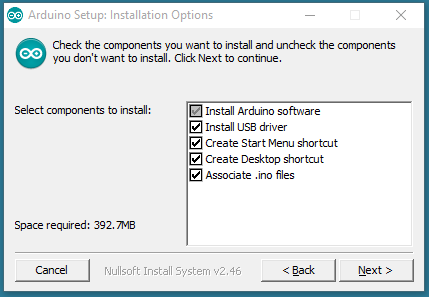
\includegraphics[width=1\textwidth]{figures/ide1.png}
\caption{Tampilan Jendela Instalasi}
\label{print}
\end{figure}
\par Pilih komponen yang sudah diinstal. Sesuaikan dengan kebutuhan anda, pastikan pilihan install USB driver telah tercentang karena ini terkait nanti dengan driver usb Arduino. Setelah beres klik Next.

\item Pada jendela berikutnya akan ditampilkan pada jendela dialog tujuan instalasi dari arduino IDE. Pilih default saja dan langsung klik Install.
\begin{figure}[H]
\centering
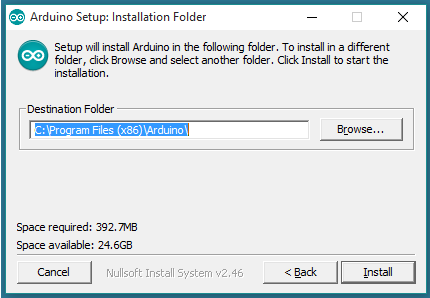
\includegraphics[width=1\textwidth]{figures/ide2.png}
\caption{Jendela Dialog Tujuan Instalasi Dari Arduino IDE }
\label{print}
\end{figure}

\begin{figure}[H]
\centering
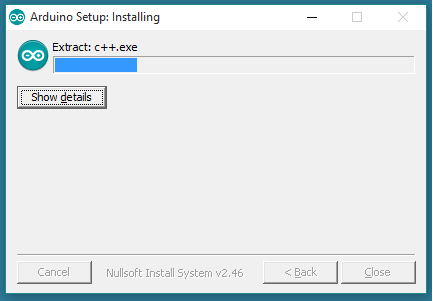
\includegraphics[width=1\textwidth]{figures/ide3.png}
\caption{Jendela Instalasi Arduino IDE }
\label{print}
\end{figure}
\end{enumerate}
\par Tunggu hingga proses instalasi selesei. Setelah Arduino IDE selesei terinstall, kini sambungkan kabel USB Arduino  pada port USB komputer/laptop. Jika anda menggunakan file installer yang sama di tunjukan pada pembahasan sebelumnya, maka arduino akan otomatis terbaca di COMX (X adalah nomer port serial, misalkan COM1 atau COM2 dan seterusnya).

\subsection{Contoh Pemograman Arduino}
Kini saatnya menjalankan Arduino IDE, pilih File > Examples > Basic > Blink  . Maka akan muncul pada jendela yang berisi source sebagai berikut:
\begin{figure}[H]
\centering
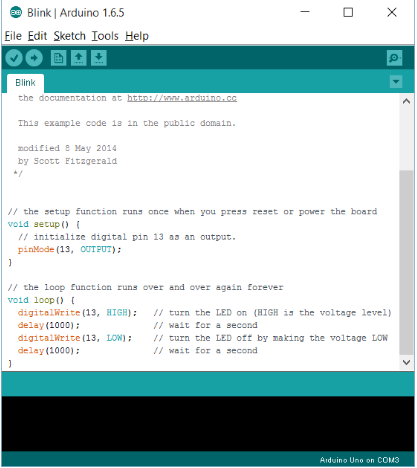
\includegraphics[width=1\textwidth]{figures/ide4.png}
\caption{Tampilan Arduino IDE Blink}
\label{print}
\end{figure}

\par Program ini memerintahkan Arduino untuk memberi sinyal digital bergantian dari  0 V dan 5V pada port 13. Kenapa Port 13? Karena di Port 13 Arduino Uno, terdapat  LED orange kecil yang tertanam dalam board sehingga untuk mengetes apakah arduino kita berfungsi atau tidak, cukup program port 13 untuk mengirimkan sinyal digital dan lihat hasilnya secara visual pada LED tersebut. Langkah selanjutnya perhatikan berikut ini :
\begin{enumerate}
    \item \textbf{Pilih Port Serial} 
    \par Sebelum kita mengupload program ke dalam board, pilih port usb dimana Arduino Uno terbaca. Pilih Tools > Port  untuk menyambungkan port.
    \item \textbf{\textit{Upload Program}}
    \par Setelah koneksi ke port serial sudah oke, klik tombol \textit{“Upload”} pada Arduino IDE. dan tunggu beberapa saat hingga muncul pesan \textit{“Done Uploading”} pada status bar. Jika berhasil, kita akan melihat LED orange arduino Uno akan berkedip-kedip dengan delay tertentu.
\par Setelah Blink kita akan membuat "Hello Word" menggunakan Arduino IDE yang nantinya akan di tampilkan di serial monitor. Berikut code pemogramannya :
\lstinputlisting{src/hello.c}
\par Setelah program diatas diketikkan pada software Arduino IDE, maka tahap selanjutnya lakukan proses \textit{Upload} kedalam board Arduinonya tunggu sampai proses selesai sampai ada tanda \textit{Done Uploading}. Untuk melihat hasilnya klik menu Tools kemudian Serial Monitor maka hasilnya akan muncul seperti gambar berikut.
\begin{figure}[H]
\centering
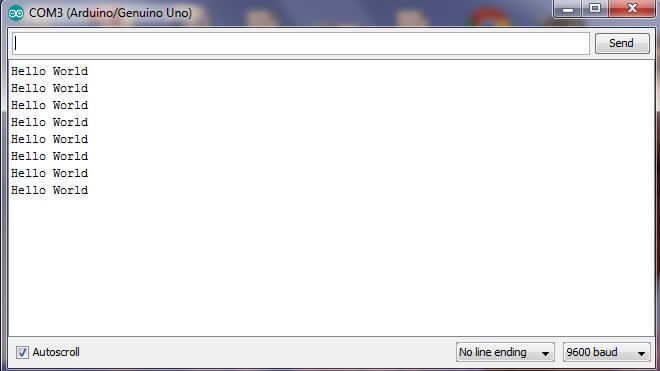
\includegraphics[width=1\textwidth]{figures/hello.jpg}
\caption{Tampilan Di Serial Monitor}
\label{print}
\end{figure}
\par Penjelasan tentang fungsi-fungsi dari tiap-tiap bagian program diatas adalah sebagai berikut:
\begin{enumerate}
    \item Void Setup()  adalah fungsi yang dijalankan secara otomatis pertama kali oleh board Arduino, dimana Semua kode program yang ada dalam void setup akan dibaca sekali oleh Arduino. Biasanya isinya berupa kode perintah untuk menentukan fungsi pada sebuah pin atau deklarasi INPUT/OUTPUT.
    \item “begin()” digunakan untuk mengatur baudrate / kecepatan transmisi data. Beberapa pilihan kecepatan komunikasi data yang dapat digunakan pada board arduino adalah 300, 1200, 2400, 4800, 9600, 14400, 19200, 28800, 38400, 57600 atau 115200. Pengaturan baudrate dilakukan pada bagian setup().
    \item Void loop() melakukan proses dimana semua kode yang ada disini akan dibaca berulang kali (terus menerus) oleh Arduino.
    \item Perintah “Serial.print” digunakan untuk menampilkan data ke serial monitor. Data yang ditampilkan dapat berupa karakter, bytes, atau angka.
    \item delay(2000) merupakan pernyataan untuk melakukan penundaan selama 2000 milidetik atau 2 detik dari proses akhir pembacaan program sebelumnya dimana Arduino akan mengulang proses pembacaan program dari awal kembali.
\end{enumerate}
\end{enumerate}
\subsection{Cara \textit{Import Library}}
\par Library adalah kumpulan code yang biasanya terkumpul dalam sebuah namespace/ module/ package (tergantung anda menggunakannya di bahasa pemrograman apa) yang dapat di import/ reuse ke program lain. Untuk mengimport library ada tiga cara yaitu menggunakan \textit{manager library}, mengimport library .zip hasil dwonload dan Instalasi Manual.
\begin{enumerate}
    \item Import Library Menggunakan Manager
\par Untuk menginstal sebuah Library baru ke dalam IDE Arduino,dapat menggunakan Library Manager (tersedia sejak Arduino IDE versi 1.6.2). Buka Arduino IDE dan klik ke menu “Sketch” dan kemudian Include Libary > Manage Libraries .
\begin{figure}[H]
\centering
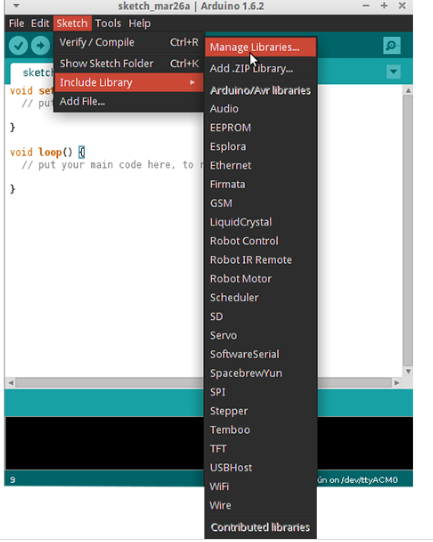
\includegraphics[width=0.7\textwidth]{figures/manager1.png}
\caption{Memilih Menu Manage Librarie}
\label{print}
\end{figure}

\par Kemudian Sketch Manager akan terbuka dan  akan menemukan daftar Library yang sudah terpasang ataupun Library baru yang siap untuk di instalasi. Dalam contoh ini kita akan menginstal library Bridge. Gulir daftar untuk menemukannya, lalu pilih versi Library yang ingin Anda instal. (beberapa Library terkadang hanya ada satu versi Library yang tersedia).
\begin{figure}[H]
\centering
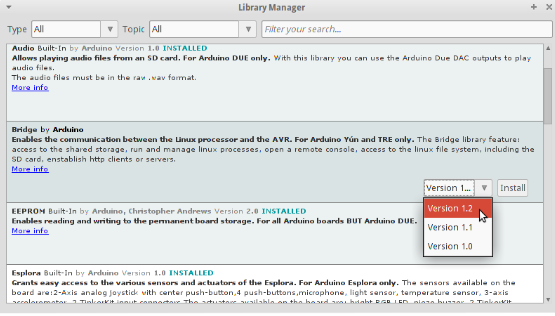
\includegraphics[width=0.9\textwidth]{figures/manager2.png}
\caption{Tampilan Sketch Manager}
\label{print}
\end{figure}
\par Langkah selanjtnya adalah klik instal dan tunggu IDE untuk menginstal library baru. Setelah selesai, sebuah tag Installed akan muncul di sebelah Library Bridge.  Setelah terinstal, sekarang kita dapat menemukan Library baru yang tersedia di menu Include Library.
\begin{figure}[H]
\centering
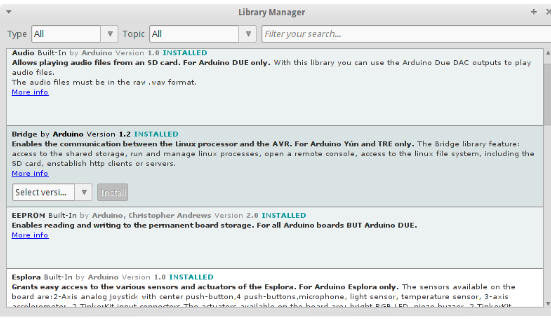
\includegraphics[width=0.9\textwidth]{figures/manager3.png}
\caption{Tampilan Library Yang Terinstall}
\label{print}
\end{figure}

\item  Mengimport Libray .zip hasil Download.

\par Terkadang Library hasil buatan sesorang banyak dan sering yang didistribusikan sebagai file ZIP atau folder sehingga dapat kita unduh, di GitHub misalnya. Nama folder adalah nama Library. Di dalam folder tersebut akan ada file .cpp, file .h , Folder Contoh Sketch, dan file lainnya yang dibutuhkan oleh Library. Dimulai dengan versi 1.0.5, Kita bisa menginstal library pihak ke-3 di IDE. Jangan unzip Libray yang telah didownload, biarkan seperti apa adanya.

\par Buka aplikasi Arduinonya, lalu Masuk ke menu SKETCH, pilih INCLUDE LIBRARY, pilih ADD. ZIP Library , seperti gambar berikut :
\begin{figure}[H]
\centering
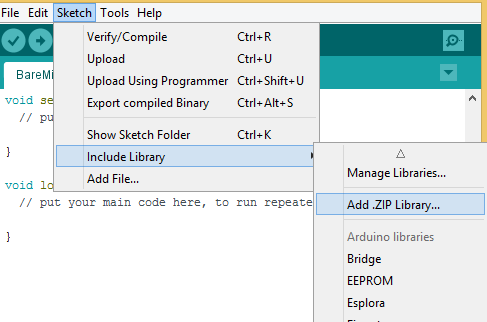
\includegraphics[width=0.7\textwidth]{figures/library1.png}
\caption{Tampilan Library ADD ZIP}
\label{print}
\end{figure}

\par Kemudian  akan diminta untuk memilih Library yang ingin ditambahkan. klik add .ZIP library, lalu cari file ZIP yang sudah didwonload.
\begin{figure}[H]
\centering
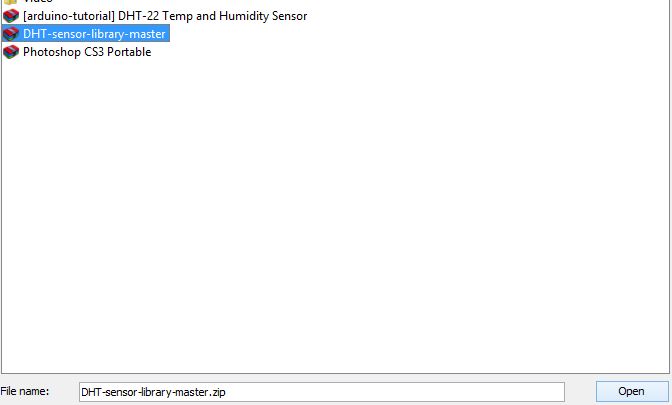
\includegraphics[width=0.9\textwidth]{figures/library2.png}
\caption{Pilih File ZIP}
\label{print}
\end{figure}

\par  Jika berhasil, aplikasi Arduino kamu akan muncul keterangan seperti dibawah ini:
\begin{figure}[H]
\centering
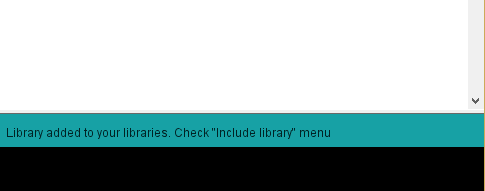
\includegraphics[width=0.9\textwidth]{figures/library3.png}
\caption{Tampilan Library Berhasil Ditambahkan}
\label{print}
\end{figure}

\item Instalasi Manual

\par Bila ingin menambahkan Library secara manual,  perlu mendownload sebagai file ZIP, lalu extrack file tersebut. (Klik Kanan pada File ZIP lalu pilih extract to “nama file” ), setelah folder hasil extrakan tersedia, selanjutnya kita harus memasukannya kedalam folder di C:User-NamaPC-Documents-Arduino-libraries.
\end{enumerate}

\section{Memprogram Komponen \textit{Prorotype PKA}}
\par Setalah kita mengetahui cara penggunaan Arduino IDE,\textit{import library}, dan struktur pemogramannya yang telah dibahas sebelum nya maka, tahapan selanjutnya yaitu mempogram komponen untuk \textit{prototype} PKA ini. Dengan cara memprogram serta testing komponen satu persatu kemudian digabungkan menjadi kesatuan yang utuh.
\subsection{Memprogram Sensor Ultasonic}
\par komponen pertama yang akan di program atau di tes yaitu sensor ultrasonic US 100 yang nantinya berfungsi untuk membaca jarak ketinggian air. Berikut kodinganya :
\lstinputlisting{src/sensor.c}
\par Penjelasan coding diatas yaitu :
\begin{enumerate}
    \item #define triggerPin  D4 #define echoPin D3
\par Script tersebut untuk menginsiasi pin yang akan digunakan. Pin D4 digunakan untuk pin trigger dan D3 digunakan untuk pin echo.
\item Serial.begin (9600); ,pinMode(triggerPin, OUTPUT); ,pinMode(echoPin, INPUT); 
\par Script diatas berada di fungsi void setup(). Serial.begin() digunakan untuk memulai serial. selanjutnya pinMode digunakan untuk menentukan fungsi dari pin yang akan digunakan (triggerPin dan echoPin). triggerPin berfungsi sebagai pin output sedangkan echoPin sebagai pin input.
\item long duration, jarak;
\par Script diatas digunakan untuk deklarasi variabel duration dan jarak. Duration dan jarak merupakan variabel bertipe long. Long merupakan tipe data serupa dengan int tetapi memiliki range yang lebih panjang.
\item   digitalWrite(triggerPin, LOW);,  delayMicroseconds(2);,  digitalWrite(triggerPin, HIGH);,  delayMicroseconds(10);  digitalWrite(triggerPin, LOW);
\par Script tersebut menjelaskan bahwa pin trigger menembakkan pulsa sinyal ultrasonik selama 10 micro second.
\item duration = pulseIn(echoPin, HIGH);
\par Selanjutnya ketika gelombang ultrasonik itu ditangkap kembali setiap pulsanya oleh pin echo maka waktu tangkap tersebut diubah menjadi variabel duration.
\item jarak = (duration/2) / 29.1;
\par Dengan persamaan diatas nilai waktu duration akan dikonversi menjadi nilai jarak dalam bentuk cm.
\item Serial.println("jarak :");,
  Serial.print(jarak);,
  Serial.println(" cm");,
  delay(1000);
\par Selanjutnya nilai jarak yang didapatkan akan ditampilkan di serial monitor setiap 1 detik (delay(1000)).

\end{enumerate}
\par Untuk melihat hasil pembacaan sensor lewat serial monitor pada arduino IDE. Jika sukses maka akan seperti gambar berikut :
\begin{figure}[H]
\centering
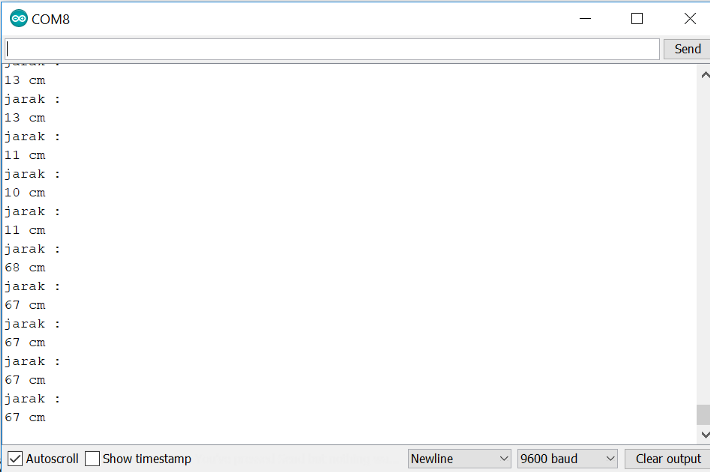
\includegraphics[width=0.9\textwidth]{figures/hasilsensor.png}
\caption{Tampilan serial monitor}
\label{print}
\end{figure}

\subsection{Memprogram Led}
\par Komponen kedua yang akan di program atau di tes yaitu led yang nantinya  berfungsi untuk sebagai indikator.Berikut Kodingannya :
\lstinputlisting{src/led.c}
\par Penjelasan coding diatas yaitu :
\begin{enumerate}
    \item const int ledPin = D2;
    \par Script tersebut untuk menginsiasi pin yang akan digunakan.
    \item pinMode(2, OUTPUT); 
    \par Menetapkan pin GPIO 2/LED sebagai OUTPUT.
    \item digitalWrite(2, LOW);
    \par  Perintah untuk mematikan Lampu atau memberikan nilai LOW(0) pada pin GPIO 2.
    \item delay(1000); 
    \par Matikan lampu selama 1 detik.
    \item digitalWrite(2, HIGH);
    \par Perintah memberikan nilai HIGH atau menyalakan Lampu.
    \item delay(2000);
    \par Nyalakan lampu selama 2 detik.
\end{enumerate}
\subsection{Memprogram Buzzer}
\par Komponen ketiga yang akan di program atau di tes yaitu buzzer yang nantinya  berfungsi untuk sebagai indikator.Berikut Kodingannya :
\lstinputlisting{src/buzzer.c}
\par Penjelasan coding diatas yaitu :
\begin{enumerate}
    \item const int ledPin = D1;
    \par Script tersebut untuk menginsiasi pin yang akan digunakan.
    \item pinMode(1, OUTPUT); 
    \par Menetapkan pin GPIO 1/Buzzer sebagai OUTPUT.
    \item digitalWrite(2, LOW);
    \par  Perintah untuk mematikan Buzzer atau memberikan nilai LOW(0) pada pin GPIO 1.
    \item delay(1000); 
    \par Matikan buzzer selama 1 detik.
    \item digitalWrite(1, HIGH);
    \par Perintah memberikan nilai HIGH atau menyalakan buzzer.
    \item delay(2000);
    \par Nyalakan buzzer selama 2 detik.
\end{enumerate}

\subsection{Memprogram Sensor, Led dan Buzzer}
\par Setelah memprogram komponen satu persatu maka selanjutnya menggabungkan komponen yang telah diprogram sebelumnya. Komponen yang akan digabungkan yaitu sensor, led , buzzer terlebih dahulu. Mengapa kita harus memprogram satu persatu terlebih dahulu tidak langsung ? alasan terlebih dahulu memprogram komponen satu persatu yaitu jika adanya error pada saat prosses penggabungan komponen akan mengetahui komponen manakah yang error. Berikut codingan dari komponen yang digabungkan :
\lstinputlisting{src/gabung.c}
\par Penjelasan coding diatas yaitu :
\begin{enumerate}
\item const int trigPin = 2;  //D4 ,
const int echoPin = 0;  //D3 ,
const int ledPin = 4;  //D2, 
const int buzzerPin = 5;  //D1
\par Script tersebut untuk menginsiasi pin yang akan digunakan. Pin D4 digunakan untuk pin trigger,D3 digunakan untuk pin echo, D2 digunakan untuk ledppin, dan D1 digunakan untuk buzzerpin.

\item // defines variables ,
long duration; ,
int distance;, 
int safetyDistance;
\par Script diatas merupakan sebuah pendefinisian variabel.
\item pinMode(trigPin, OUTPUT);,
pinMode(echoPin, INPUT); ,
pinMode(buzzerPin, OUTPUT); ,
pinMode(ledPin, OUTPUT);,
Serial.begin(115200); 
\par Pada script tersebut merupakan sebuah bagian void setup yang berfungsi sebagai output dan input dari komponen. Selain itu pada script tersebut adanya baudrate yang digunakan 115200 yang berfungsi untuk komunisai serial.

\item digitalWrite(trigPin, LOW); ,
delayMicroseconds(2);

\par Script diatas merupakan sebuah perintah untuk mematikan (\textit{Low} pada trigpin disensor ultrasonic.

\item digitalWrite(trigPin, HIGH ,
delayMicroseconds(10); ,
digitalWrite(trigPin, LOW);
 
 \par Pada bagian script diatas merupakan sebuah perintah untuk trigpin pada sensor ultrasonic dan akan adanya jeda sebesar 10 detik.
 
 \item safetyDistance = distance;//
if (safetyDistance <= 5){//
  digitalWrite(buzzerPin, HIGH);//
  digitalWrite(ledPin, HIGH);//
}//
else{//
  digitalWrite(buzzerPin, LOW);//
  digitalWrite(ledPin, LOW);//
}
\par Script tersebut merupakan sebuah logika dari sensor ultrasonic. Dimana jika jarak yang dibaca oleh sensor ultrasonic adalah kurang dari sama dengan 5  maka buuer dan led akan menyala dan jika tidak membaca jarak kurang sama dengan 5 buzzr dan led mati.

\item Serial.print("Distance: "); ,
Serial.println(distance); ,
Serial.print("pulseIn "); ,
Serial.print("duration "); ,

\par Bagian script tersebut merupakan sebuah komunkasi serial yang nantinya jarak yang dibaca oleh sensor akan di tampilkan di serial monitor.
\end{enumerate}
\subsection{Memprogram Komponen dan Antares}
Setelah semua komponen yang digabungkan sudah diprogram maka tahapan selanjutnya yaitu menambahkan pemograman untuk antaresnya. Antares tersebut akan digunakan sebagai media penyimpan data yang dibaca oleh sensor ultrasonic. Sebelum memprogram ada langkah-langkah yang harus dilakukan untuk tahapan antares ini yaitu :
\begin{enumerate}
    \item Registrasi di Antares menggunakan gmail. Untuk membuka halaman antares cukup ketikan https://antares.id/id/index.html pada browser maka akan muncul tampilan seperti gambar berikut.
    \begin{figure}[H]
    \centering
    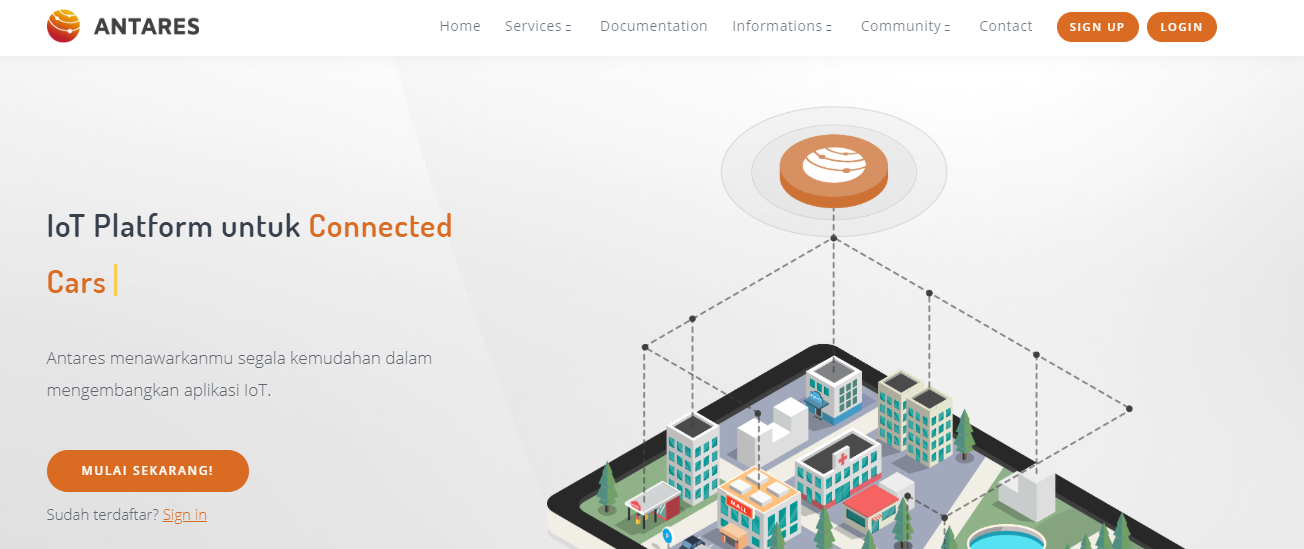
\includegraphics[width=1\textwidth]{figures/antares2.png}
    \caption{Halaman Awal Antares}
    \label{print}
    \end{figure}
    \par Setelah halaman tersebut muncul, pilih \textit{Signup} kemudian masukan email yang aktif.
    \begin{figure}[H]
    \centering
    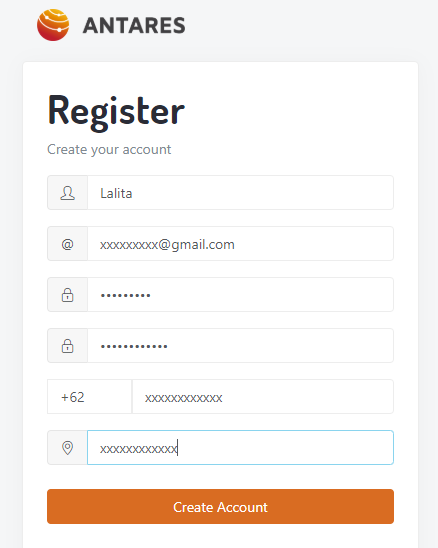
\includegraphics[width=1\textwidth]{figures/antares3.png}
    \caption{Tampilan Registrasi Antares}
    \label{print}
    \end{figure}
    \par Masukan nama , alamat email (alamat email aktif), password, no telepon dan alamat. Alamat email harus aktif karena ini berguna untuk \textit{verifikasi account} dan apabila ada info mengenai antares akan dikirmkan melalui email. 
    
    \begin{figure}[H]
    \centering
    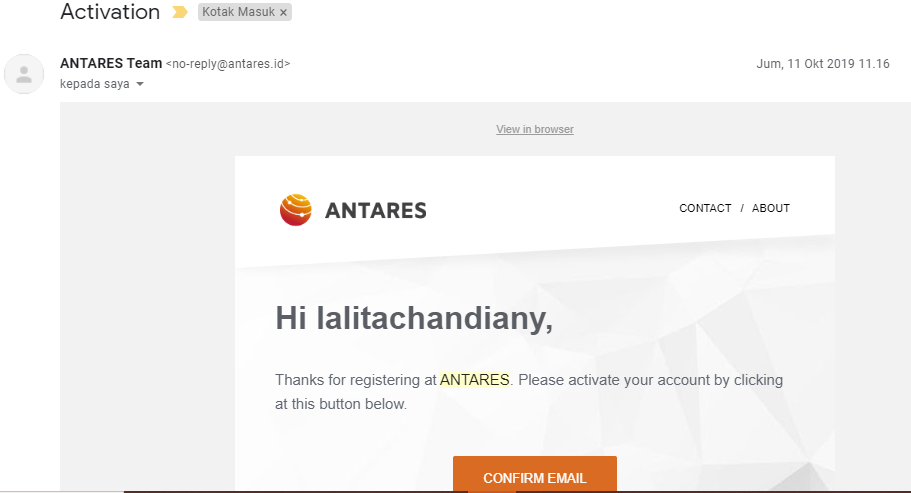
\includegraphics[width=1\textwidth]{figures/antares4.png}
    \caption{Verifikasi email}
    \label{print}
    \end{figure}
    
    \par Setelah melakukan registrasi di antares maka akan adanya email \textit{verifikasi} pada email yang sebelumnya email tersebut di daftarkan. Untuk mengkonfirmasi \textit{verifikasi} dari pihak antares cukup klik \textit{confirm}
    \begin{figure}[H]
    \centering
    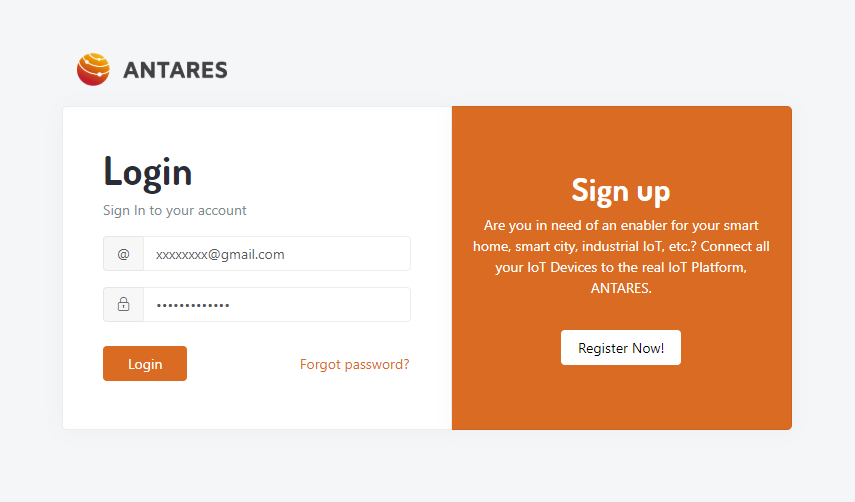
\includegraphics[width=1\textwidth]{figures/antares5.png}
    \caption{Login Antares}
    \label{print}
    \end{figure}
    \par setelah kita meng\textit{confirm} antares di email maka kita harus login di antares dengan mamasukan email yang telah didaftarkan dan memasukan password yang sebelumnya telah dibuat.
    
    \begin{figure}[H]
    \centering
    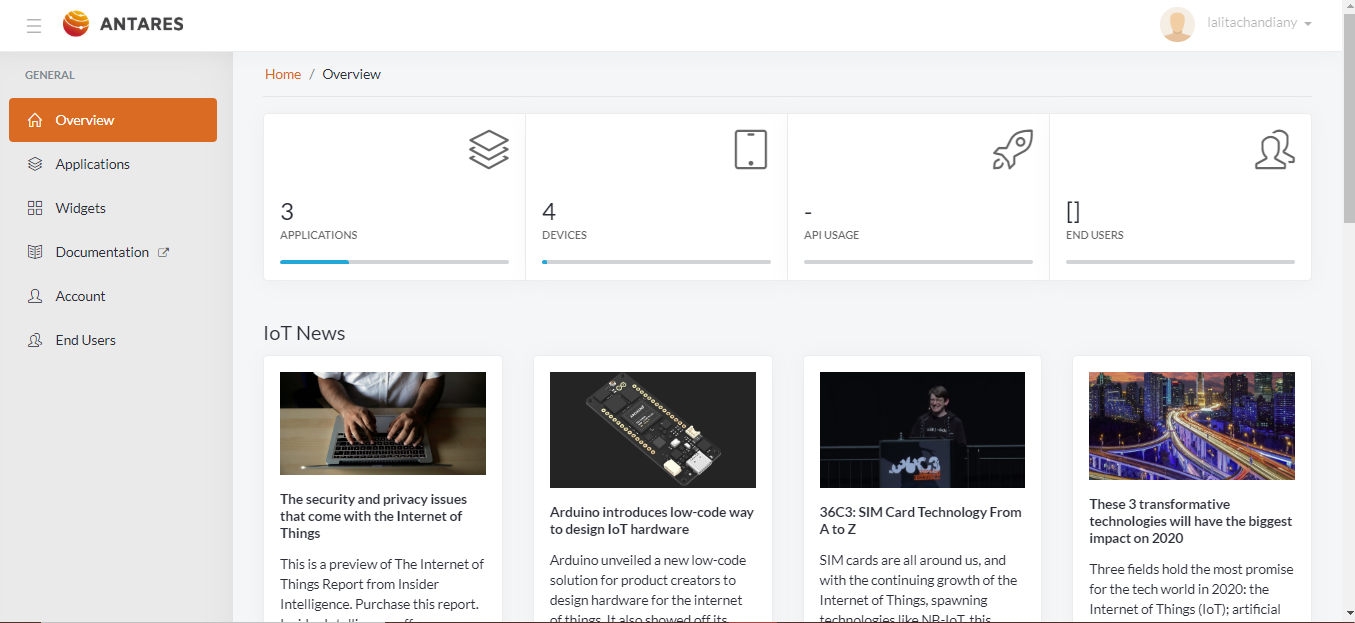
\includegraphics[width=1\textwidth]{figures/antares6.png}
    \caption{Tampilan Awal Antares}
    \label{print}
    \end{figure}
    
    \par Gambar diatas merupakan halaman awal antares ketika kita sudah login. Dalam halaman ini adanya beberapa menu yaitu :
    \begin{enumerate}
        \item \textit{Overview}
        \item \textit{Application}
        \item \textit{Widgets}
        \item \textit{Documentation}
        \item \textit{Account}
        \item \textit{Enduser}
    \end{enumerate}
     \begin{figure}[H]
    \centering
    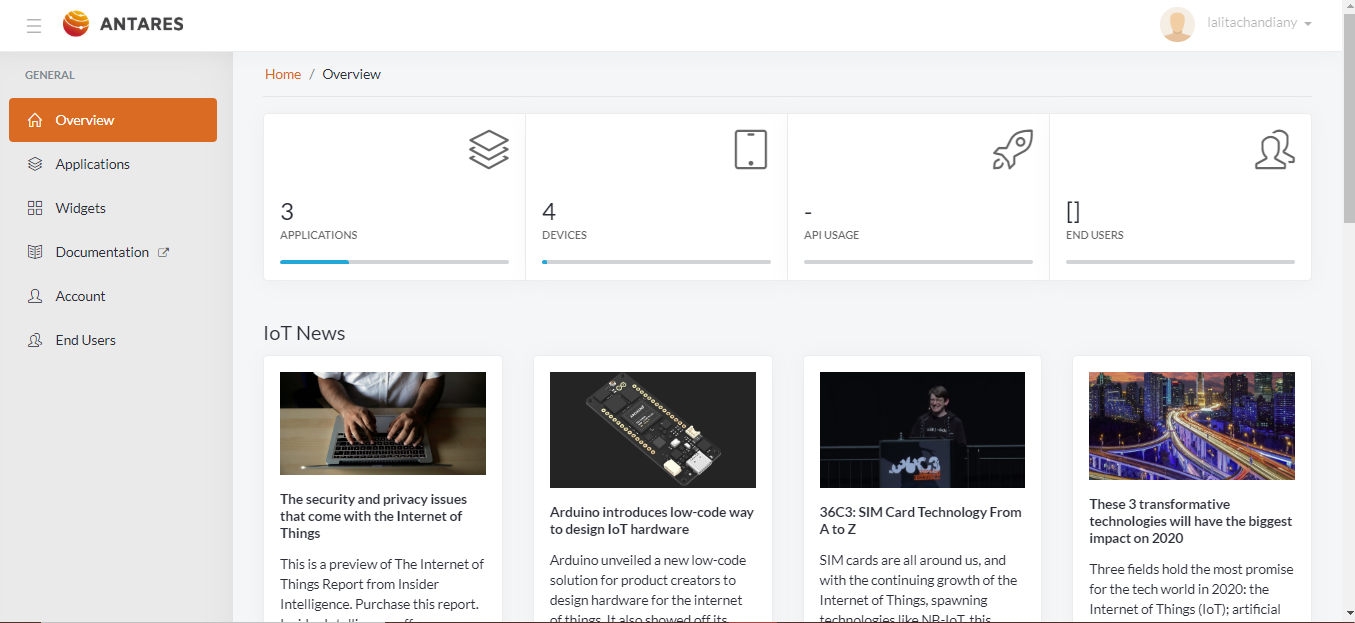
\includegraphics[width=1\textwidth]{figures/antares6.png}
    \caption{Halaman \textit{Overview}}
    \label{print}
    \end{figure}
    \par Halaman \textit{Overview} merupakan halaman awal yang ditampilkan pada saat setelah login. Halaman ini menampilkan sebuah berita mengenai IoT (\textit{Internet of Thing)}. Selain mengenai berita IoT halaman ini juga menampikan project yang sudah kita buat. Adanya \textit{application, device, API useage dan enduser.}
    \begin{figure}[H]
    \centering
    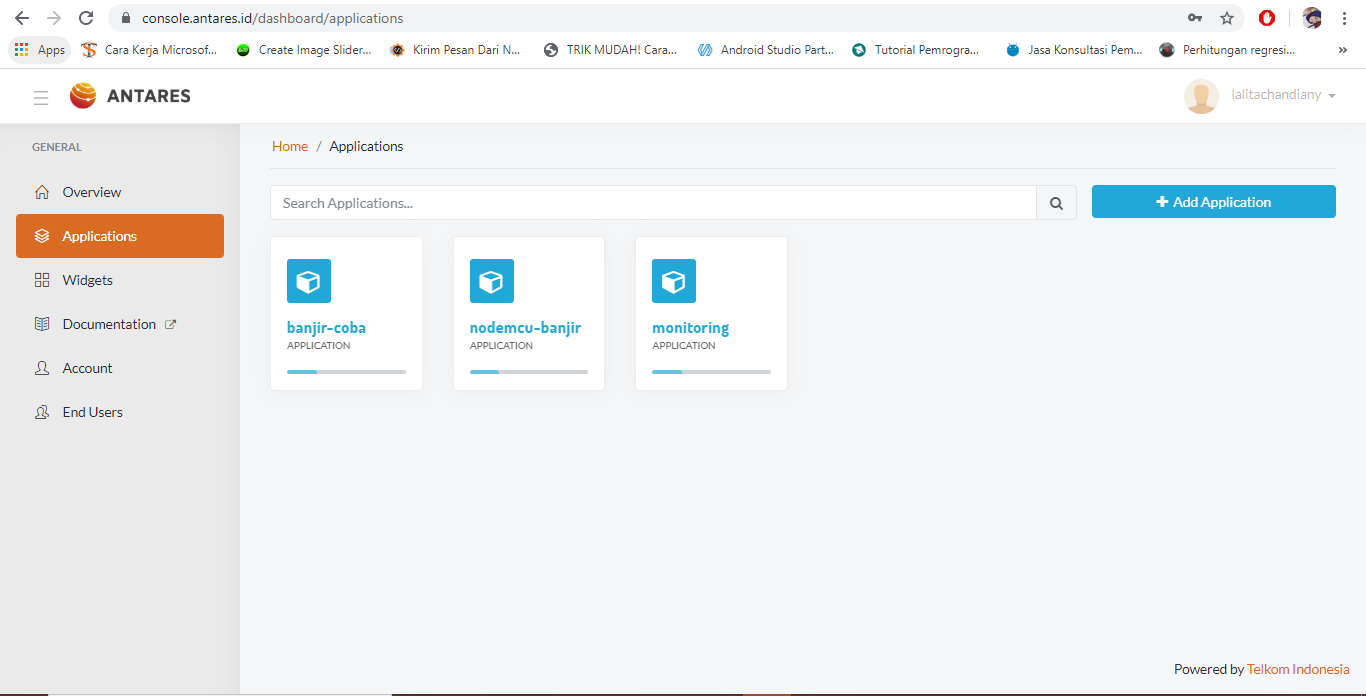
\includegraphics[width=1\textwidth]{figures/antares7.png}
    \caption{Halaman \textit{Apllication}}
    \label{print}
    \end{figure}
    \par Pada halaman \textit{application} menapilkan \textit{project} yang telah dibuat. Kemudian pada halaman ini kita dapat membuat sebuah project baru.
      \begin{figure}[H]
    \centering
    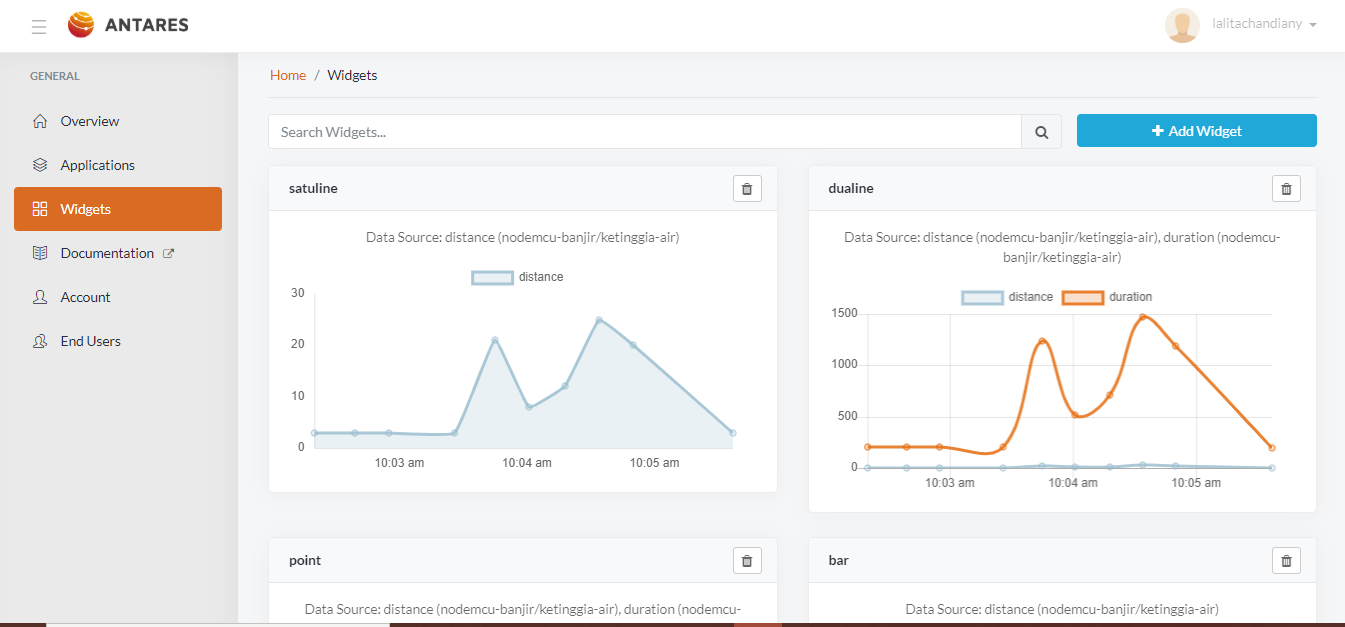
\includegraphics[width=1\textwidth]{figures/antares8.png}
    \caption{Halaman \textit{Widgets}}
    \label{print}
    \end{figure}
    
    \par Halaman widget merupakan sebuah halaman yang menampilkan sebuah grafik yang telah dibuat sebelumnya. Selain menampilkan sebuah grafik dalam halaman ini dapat membuat sebuah grafik baru.
     \begin{figure}[H]
    \centering
    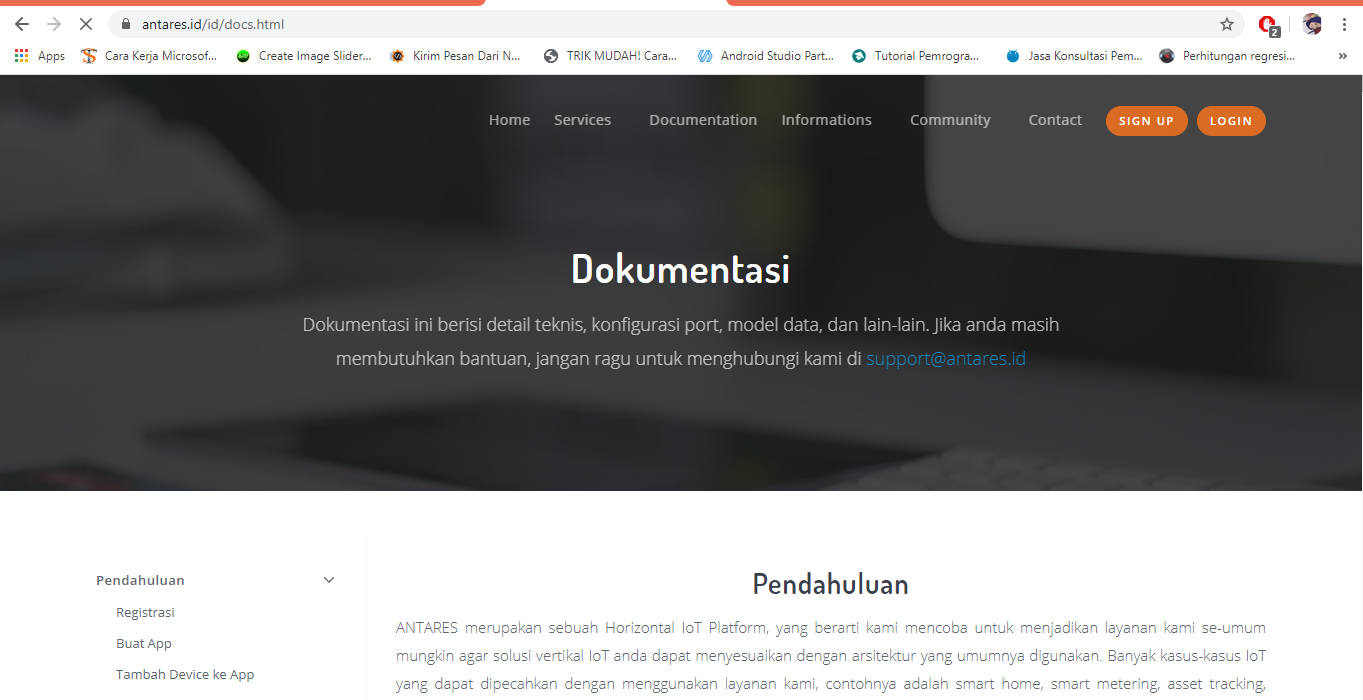
\includegraphics[width=1\textwidth]{figures/antares9.png}
    \caption{Halaman \textit{Documentation}}
    \label{print}
    \end{figure}
    
    \begin{figure}[H]
    \centering
    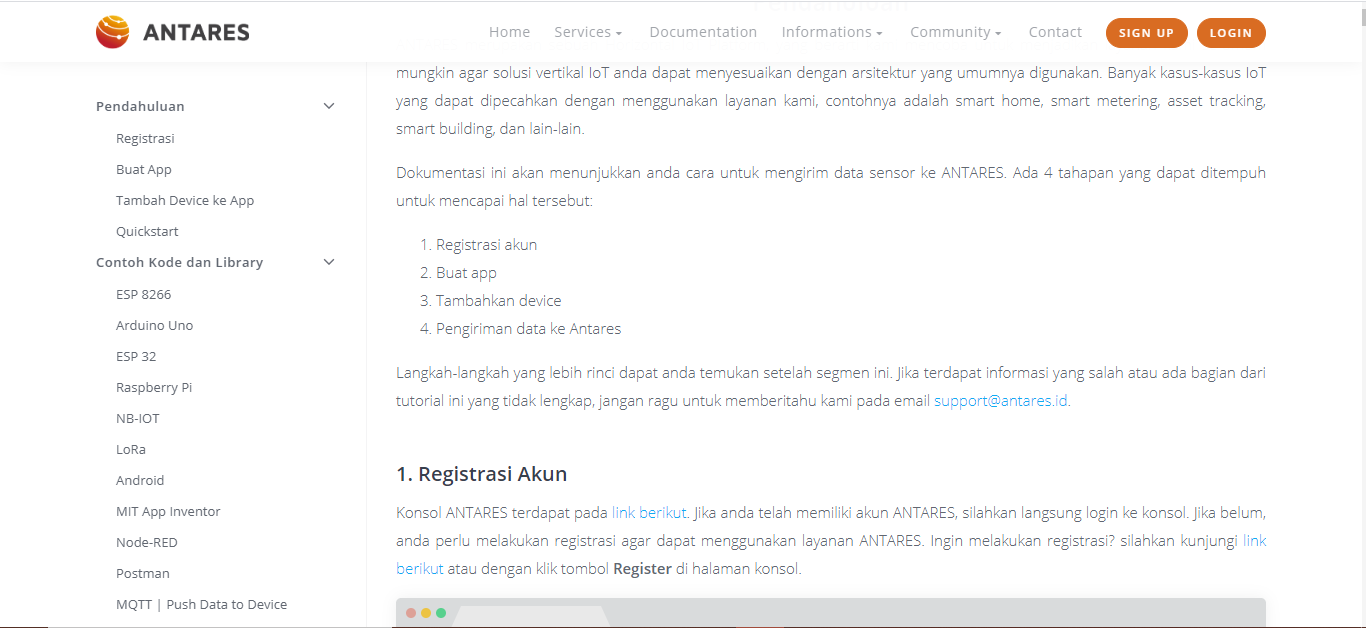
\includegraphics[width=1\textwidth]{figures/antares10.png}
    \caption{Halaman \textit{Documentation}}
    \label{print}
    \end{figure}
    \par Halaman \textit{Documentation} ini merupakan sebuah halaman yang menampilkan tutorial atau penjelasan mengenai penggunaan antares.
    \begin{figure}[H]
    \centering
    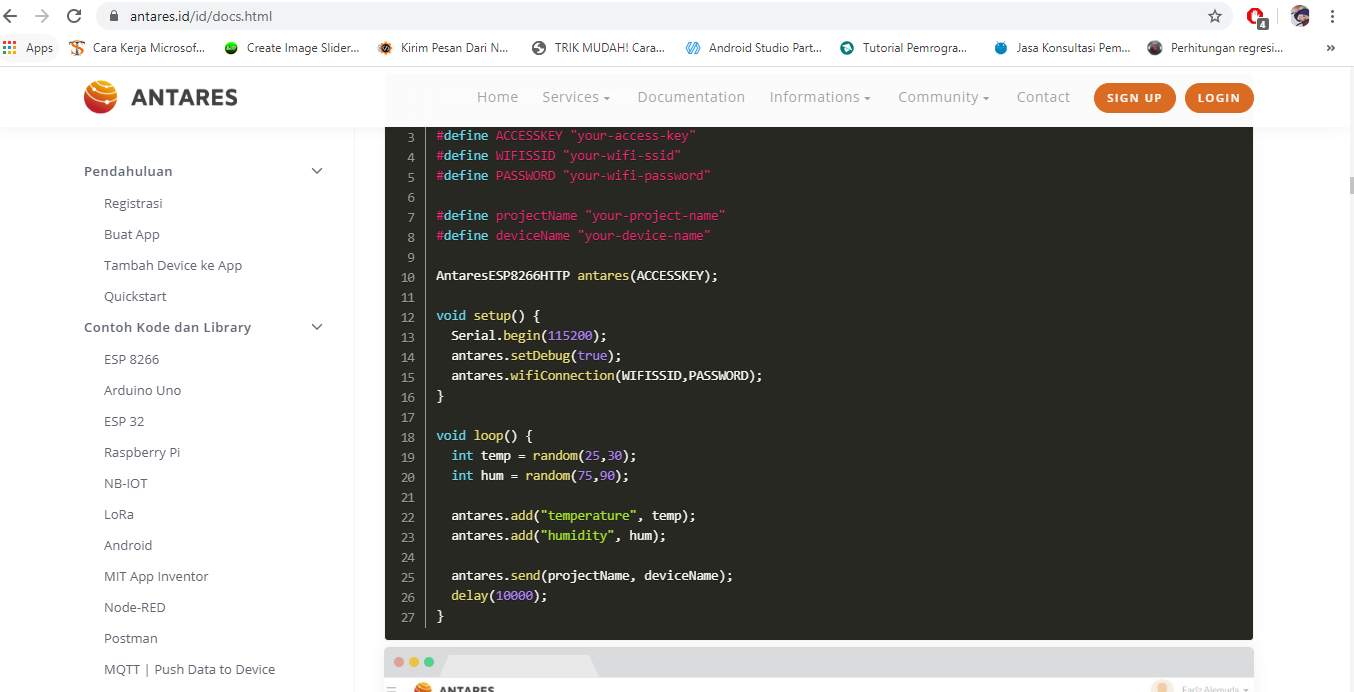
\includegraphics[width=1\textwidth]{figures/antares11.png}
    \caption{Halaman \textit{Documentation} Tutorial}
    \label{print}
    \end{figure}
    
       \begin{figure}[H]
    \centering
    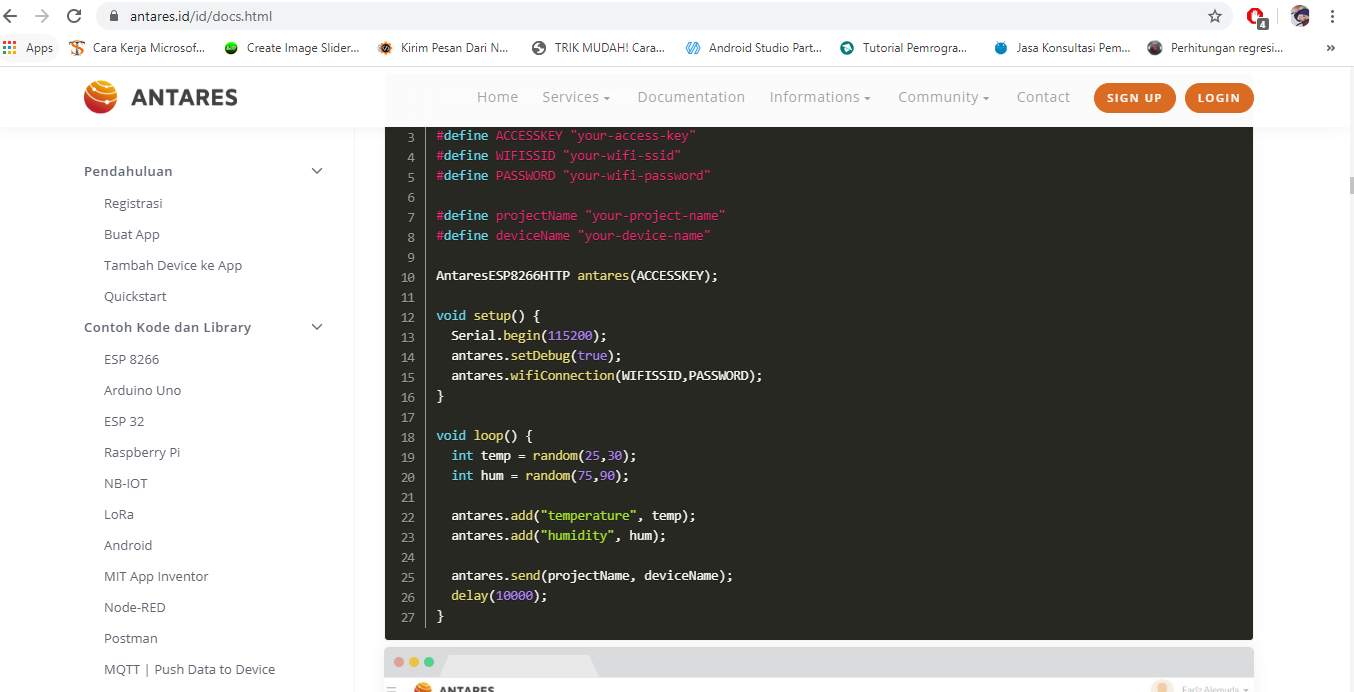
\includegraphics[width=1\textwidth]{figures/antares11.png}
    \caption{Halaman \textit{Documentation}Tutorial}
    \label{print}
    \end{figure}
    \par Pada halaman \textit{documentation} juga terdapat sebuah tutorial mengenai komponen yang dimana menggunakan antares sebagai media penyimpanan datanya. Kemudian pada halaman ini juga menampilkan sebuah contoh kode library yang bisa kita gunakan.
\end{enumerate} 